\section{Algoritmi di Scheduling}
\subsection{Introduzione}
\subsubsection{Obiettivi dello scheduling}
Un sistema operativo deve gestire molti processi contemporaneamente, ma la CPU può eseguirne solamente uno alla volta. Introduciamo quindi il concetto di scheduling il quale consiste nel decidere quale processo deve essere eseguito in un dato istante. Lo scheduling ha come obiettivo, quindi, quello di ottimizzare l'utilizzo della CPU trovando un bilanciamento tra:
\begin{itemize}
    \item massimizare il throughput: quanti processi sono eseguiti
    \item minimizzare la latenza: quanto tempo un processo aspetta per essere eseguito
    \item starvation: evitare che un processo non venga mai eseguito
    \item completare una processo entro un tempo predefinito
    \item massimizzare la percentuale di utilizzo del processore
\end{itemize}
\subsubsection{Preemption}
Introduciamo, inoltre, il concetto di preemption il quale indica se un algoritmo di scheduling e/o un processo è interrompibile o meno. Ci sono due possibilità inerenti al preemption:
\begin{itemize}
    \item la politica preemptive: 
    \begin{enumerate}
        \item un processo può essere interrotto per farne eseguire un altro, di conseguenza un processo non deve aspettare la terminazione di quello corrente prima di essere eseguito
        \item i processi interrotti aspettano che vengano eseguiti in memoria
        \item in ambienti multiprocessore un processo può essere rimosso dalla CPU alla quale è stato assegnato per effettuare un load balancing
        \item ha un costo maggiore in quanto la CPU deve tenere traccia dei processi in attesa, quindi salvare gli stati dei processi al tempo della interruzione, e avere un meccanismo che possa cambiare tra un processo all'altro
    \end{enumerate}

    \item la politica nonpreemptive:
    \begin{enumerate}
        \item un processo viene eseguito dall'inizio alla fine senza cedere il controllo della CPU a prescindere dalla durata o dalla priorità di altri processi in arrivo
        \item è rischioso in quanto un processo potrebbe bloccarne un altro per un tempo indefinito
        \item ha un costo minore in quanto non bisogna tenere traccia degli stati correnti dei processi in attesa e non c'è un sovraccarico della CPU con il cambio di processo
    \end{enumerate}
\end{itemize}

\subsubsection{Politiche degli algoritmi di scheduling}
Lo scheduling, quindi, è effettuato da un componente chiamato scheduler che, decide l'ordine temporale per il quale i processi devono accedere alla CPU. Esistono vari modi per scegliere l'ordine temporale e questo dipende da diversi fattori quali:
\begin{enumerate}
    \item la priorità del processo
    \item l'arrivo temporale della richiesta del processo
    \item la durata del processo
    \item il tempo di attesa in coda
\end{enumerate}
Le politiche di scheduling sono innumerevoli, ma tutti hanno come unico obiettivo quello di ottimizzare il rendimento della CPU. In particolare sono comuni a tutti gli algoritmi di scheduling l'equità, la scalabilità e la predicibilità, ovvero tutti i processi con le stesse caratteristiche sono tratti in maniera uguale che non varia dal numero dei processi da schedulare e, sapendo la politica adottata, si può risalire al risultato finale. Infine, in base a quali sono le caratteristiche che si vogliono rispettare, l'algoritmo di scheduling può essere più o meno complesso.
\subsection{Algoritmi di Scheduling in OS161}
Lo scheduler della versione base di OS161 offre un algoritmo di Round Robin con politica preemptive. Prima di esaminare in dettaglio il codice del sistema operativo spieghiamo brevemente il funzionamento dell'algoritmo in questione.
\subsubsection{Algoritmo di Round Robin}
Lo scheduling Round Robin è un algoritmo che si basa sulla divisione della durata dei processi in piccole porzioni chiamate quanta (il plurale di quantum) che vengono eseguite ciclicamente in base all'ordine di arrivo e senza concetto di priorità.
\begin{figure}[hbt!]
    \centering
    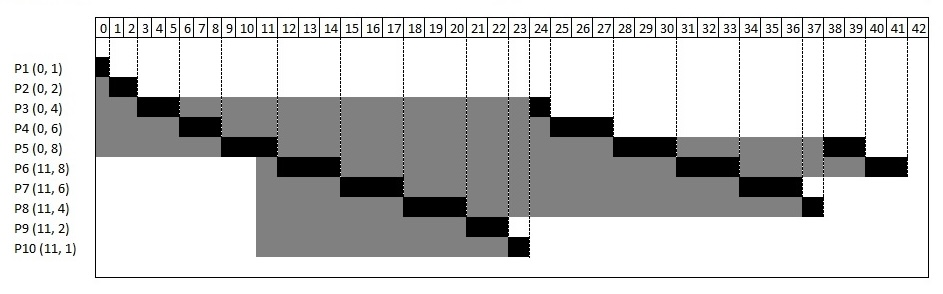
\includegraphics[width=\textwidth]{Algoritmi di Scheduling/images/round_robin.jpg}
    \caption{Rappresentazione temporale di uno scheduling round robin. In questo esempio i processi sono descritti da una coppia di valori che rappresentano il tempo di arrivo e la durata. Il time quantum è di 3 unità temporali e l'area grigia rappresenta il tempo di attesa di un processo prima di essere stato eseguito completamente.}
    \label{round_robin}
\end{figure}

Come possiamo notare dalla figura, è uno scheduling di tipo preemptive in quanto ogni quantum di tempo passato, se il processo in corso non è terminato viene sospeso e si passa al successivo. I processi aspettano in una coda ordinata in base al tempo di arrivo, i processi che devono essere eseguiti vengono estratti da questa coda e vengono eliminati da essa solamente una volta terminati completamente. Infine, è anche starvation free in quanto tutti i processi hanno la stessa priorità e possibilità di essere eseguiti a prescindere dalla durata di essi.

\subsubsection{Scheduler in OS161}
Una volta esaminato il comportamento ad alto livello dello scheduler, passiamo a studiare il funzionamento a basso livello.

I principali dettagli implementativi dell'algoritmo sono descritti in \lstinline{kern/thread/clock.c} in cui troviamo la definizione temporale
\begin{lstlisting}[caption={Vincoli temporali in \lstinline{clock.c}}]
#define SCHEDULE_HARDCLOCKS	4
#define MIGRATE_HARDCLOCKS	16
\end{lstlisting}
che rappresentano rispettivamente ogni quanti cicli di clock hardware avviene lo scheduling e la migrazione (in caso di architettura multiprocessore si può spostare il thread in un'altra CPU se sono libere o meno occupate).

Lo scheduling è gestita dalla funzione \lstinline{hardclock()} che si trova in \lstinline{kern/thread/clock.c} che a sua volta chiama la funzione per schedulare o per migrare il thread e viene chiamata un numero fisso \lstinline{HZ} di volte al secondo.
\begin{lstlisting}[caption=Quanti hardcloks al secondo in \lstinline{clock.h}]
#define HZ  100
\end{lstlisting}

Le funzioni che gestiscono lo scheduling e la migrazione del thread sono rispettivamente \lstinline{schedule()} e \lstinline{thread_consider_migration()}, in questa sezione ci concentreremo sulla prima.
La funzione che le racchiude viene chiamata (da ogni CPU) 100 volte al secondo e semplicemente incrementa il numero di cicli di clock e se è un multiplo di \lstinline{MIGRATE_HARDCLOCKS} chiama la funzione dedicata alla migrazione mentre se è multiplo di \lstinline{SCHEDULE_HARCLOCKS} viene chiamata la funzione per lo scheduling. Essa nella versione base di OS161 è vuota in quanto non è previsto nessuna forma articolata di scheduling, ma qualora si volesse implementare la si dovrebbe modificare presente in \lstinline{kern/thread/thread.c}

\begin{lstlisting}[caption={\lstinline{hardclock()} in \lstinline{clock.c}}]
void
hardclock(void)
{
	curcpu->c_hardclocks++;
	if ((curcpu->c_hardclocks % MIGRATE_HARDCLOCKS) == 0) {
		thread_consider_migration();
	}
	if ((curcpu->c_hardclocks % SCHEDULE_HARDCLOCKS) == 0) {
		schedule();
	}
	thread_yield();
}
\end{lstlisting}

L'unico scheduling effettuato dal sistema operativo è eseguito dalla funzione \lstinline{thread_yield()} che a sua volta chiama \lstinline{thread_switch(S_READY,NULL,NULL)}. Essa ha come parametro fondamentale \lstinline{S_READY} che rappresenta lo stato del thread, quindi è pronto per essere eseguito che all'interno di uno switch case, indirizzerà il thread corrente all'interno della funzione \lstinline{thread_make_runnable}.

\begin{lstlisting}[caption={La funzione \lstinline{thread_make_runnable} in \lstinline{kern/thread/thread.c}}]
static
void
thread_make_runnable(struct thread *target, bool already_have_lock)
{
	struct cpu *targetcpu;

	/* Lock the run queue of the target thread's cpu. */
	targetcpu = target->t_cpu;

	if (already_have_lock) {
		/* The target thread's cpu should be already locked. */
		KASSERT(spinlock_do_i_hold(&targetcpu->c_runqueue_lock));
	}
	else {
		spinlock_acquire(&targetcpu->c_runqueue_lock);
	}

	/* Target thread is now ready to run; put it on the run queue. */
	target->t_state = S_READY;
	threadlist_addtail(&targetcpu->c_runqueue, target);

	if (targetcpu->c_isidle && targetcpu != curcpu->c_self) {
		/*
		 * Other processor is idle; send interrupt to make
		 * sure it unidles.
		 */
		ipi_send(targetcpu, IPI_UNIDLE);
	}

	if (!already_have_lock) {
		spinlock_release(&targetcpu->c_runqueue_lock);
	}
}
\end{lstlisting}

Questa funzione semplicemente inserisce il thread nella coda dei thread in esecuzione. Come possiamo vedere nel file \lstinline{kern/include/thread_list.h} nella versione base di OS161 la coda è semplicemente una lista doppio puntata. Quindi qualora si volesse implementare un algoritmo più sofisticato all'interno del sistema operativo si dovrebbe modificare la funzione \lstinline{schedule()}, citata sopra, accedendo alla coda dei thread e modificando il loro ordine per decidere lo scheduling.

\begin{lstlisting}[caption={Struttura dati della coda dei thread in esecuzione}]
struct threadlistnode {
 struct threadlistnode *tln_prev;
 struct threadlistnode *tln_next;
 struct thread *tln_self;
};

struct threadlist {
	struct threadlistnode tl_head;
	struct threadlistnode tl_tail;
	unsigned tl_count;
};
\end{lstlisting}

\subsection{Algoritmi di Scheduling in xv6}